\Needspace{35\baselineskip}
\problem{main\_experiment}{Experiment on OWT}{2}
\label{prob:owt}

OWT used the standard TinyStories backbone, batch 16, context 256, and
80,000 updates (327.68M tokens), retaining its 32k tokenizer. Final loss
was 3.8596, also the lowest sampled value. Compared with low-resource
OWT's 4.4561, the longer recipe improved by 0.5965 nats per token.
Settings are in Appendix~\ref{app:standard_protocol}.

\begin{table}[htbp]
    \centering\small
    \begin{tabular}{@{}lrrrr@{}}
        \toprule
        Dataset & Updates & Final val loss & Best sampled loss & Time (min) \\
        \midrule
        TinyStories & 80,000 & 1.3245 & 1.3240 at 79,200 & 66.85 \\
        OWT & 80,000 & 3.8596 & 3.8596 at 80,000 & 79.45 \\
        \bottomrule
    \end{tabular}
    \caption{Standard-budget results from the saved logs. Times are the last
    logged training elapsed times, including intervening evaluation/saving but
    excluding startup and final evaluation/checkpoint overhead.}
    \label{tab:standard_results}
\end{table}

\begin{figure}[htbp]
    \centering
    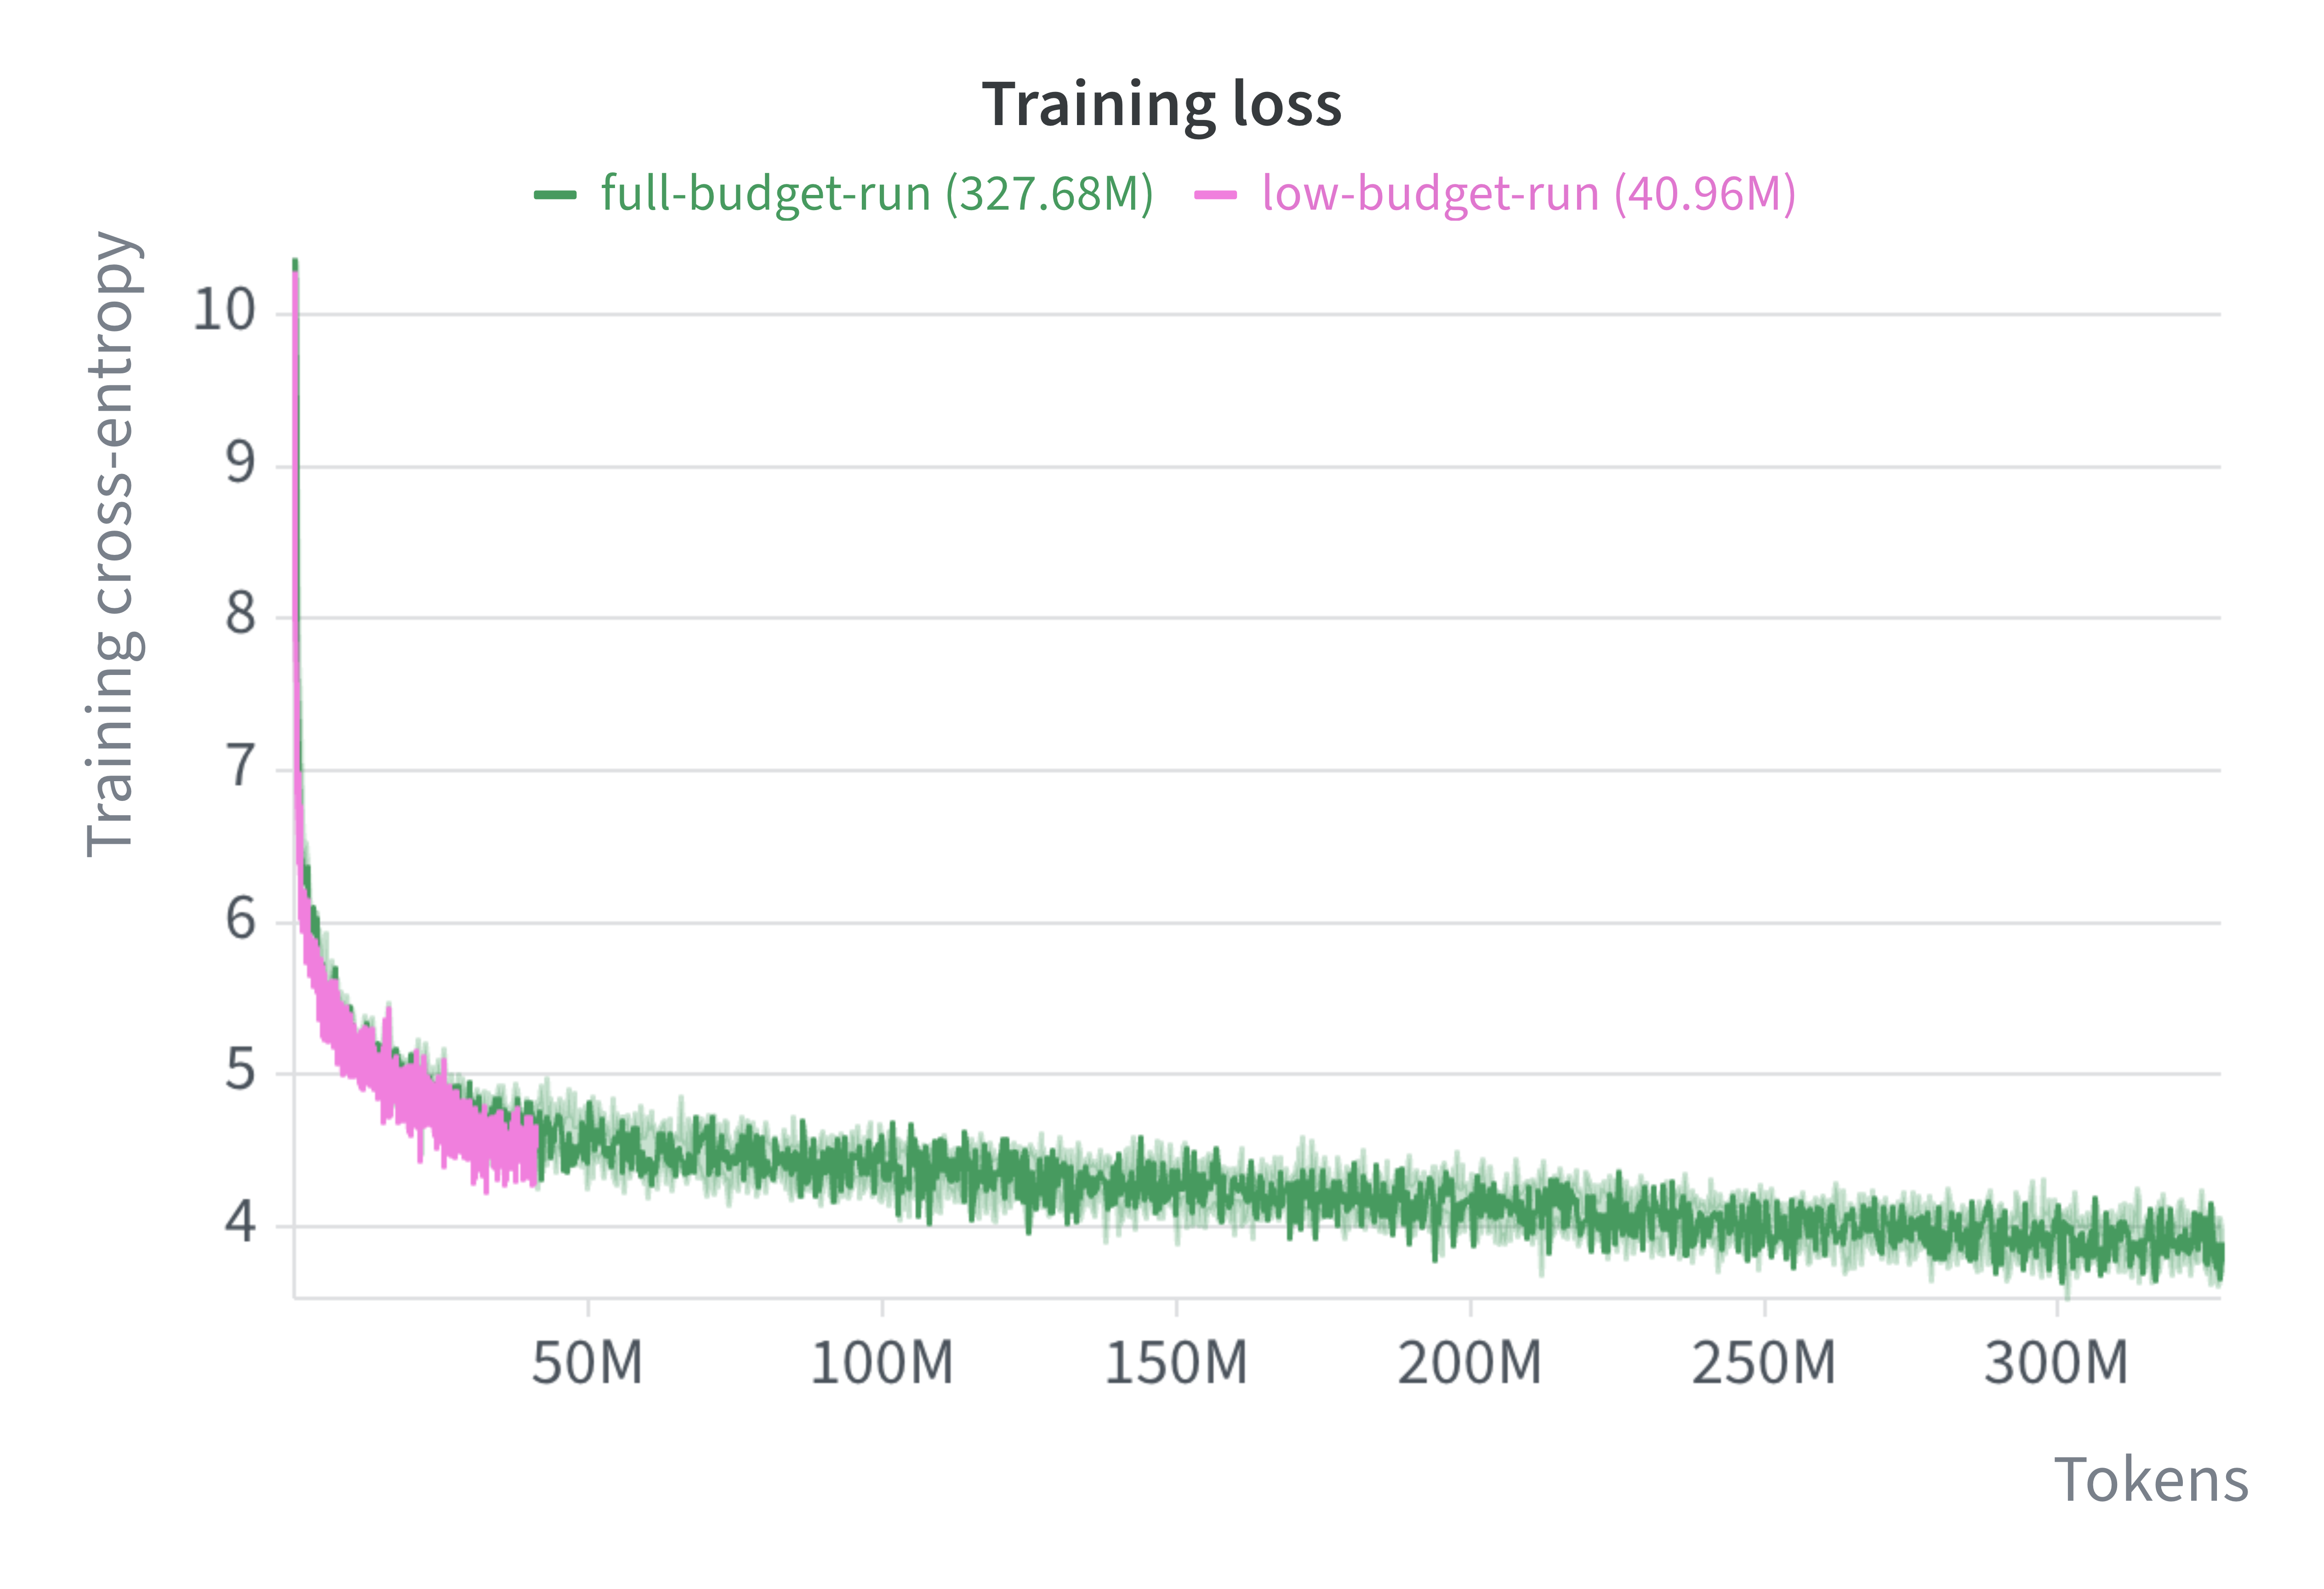
\includegraphics[width=0.49\textwidth]{figures/owt_full_train.png}\hfill
    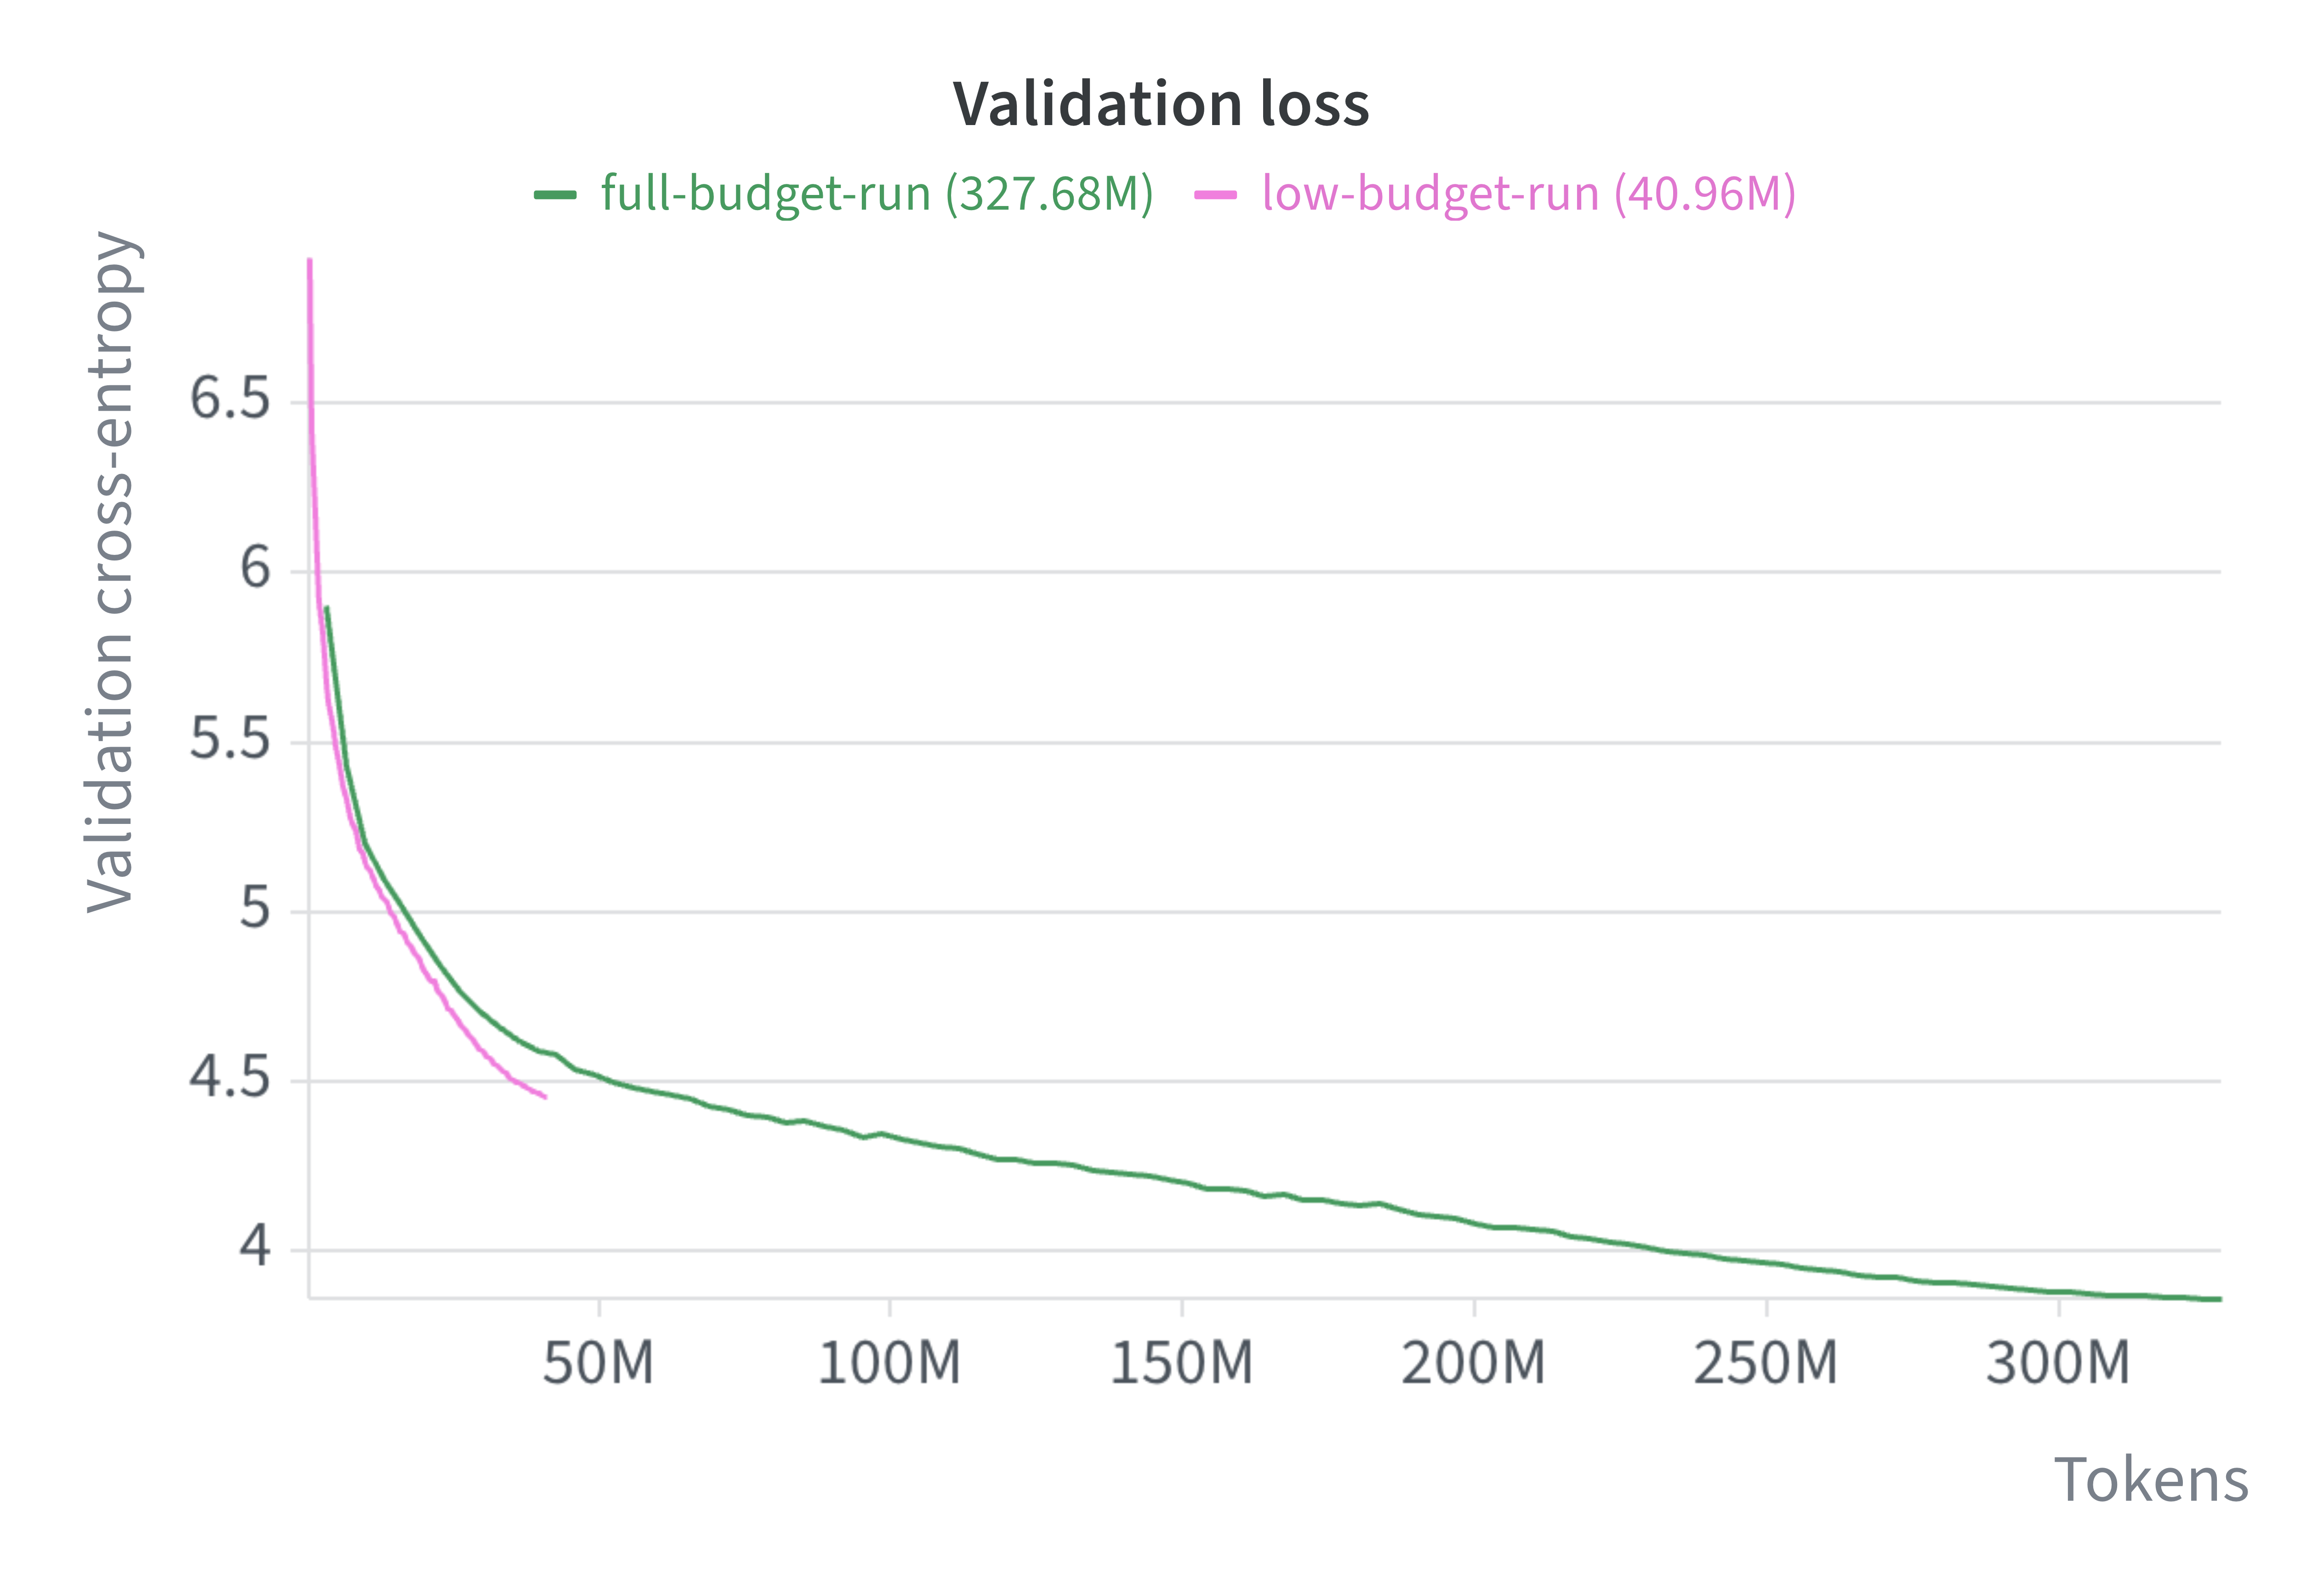
\includegraphics[width=0.49\textwidth]{figures/owt_full_val.png}
    \caption{OWT training loss (left) and fixed-window validation loss
    (right) against training tokens. Green: 327.68M; pink: 40.96M.
    Both W\&B panels use linear axes.}
    \label{fig:owt_budget}
\end{figure}

OWT's numerical loss cannot directly rank corpus difficulty against
TinyStories: the tokenizers differ, and perplexity retains this mismatch.
Within-dataset budget comparisons are more interpretable; they change
both training length and the LR schedule.

Web text spans more domains than children's stories. OWT generations
match topic/style but remain repetitive and incoherent, consistent with
limited modeling capacity at this budget. Corpus, tokenizer, and parameter
count also differ, so equal tokens do not imply equal compute or isolate
corpus complexity. See \hyperref[prob:generate]{Problem (\texttt{generate})}
for prompt comparisons and Appendix~\ref{app:standard_samples} for full outputs.
